\begin{figure}[H]
    \centering
    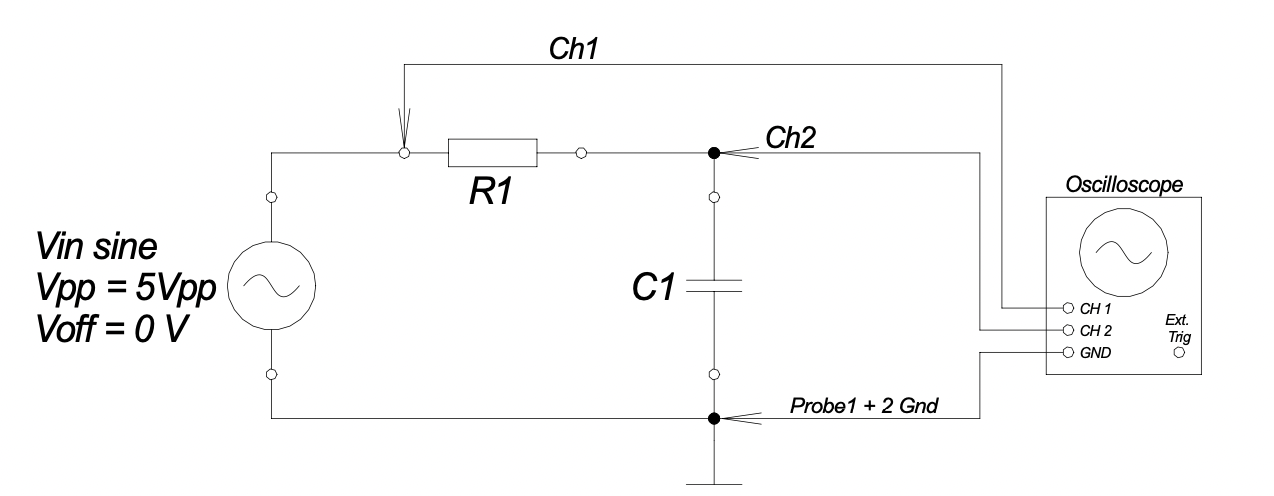
\includegraphics[scale=0.5]{images/part1_circuit.png}
    \caption{$C_1$ = 1.5nF and $R_1$ = 22K$\Omega$}
\end{figure}


The signal generator is connected via the BNC-To-Kleps cable. The CH1 channel is used for the input, and the CH2 channel is used for the output.
The frequency at the signal generator is then varied in steps of 1, 2, 5, 10 steps up to 100KHz.

\begin{adjustwidth}{-2.5 cm}{-2.5 cm}\centering\begin{threeparttable}[!htb]
        \scriptsize
        \begin{tabular}{lrrrrr}\toprule
            \textbf{Input Voltage(in V)} & \textbf{Output Voltage(in V)} & \textbf{Phase(in deg)} & \textbf{Frequency(in Hz)} & \textbf{Amplitude(in dB)} \\\midrule
            10.1                         & 10                            & -0.36                  & 50                        & -0.09                     \\
            10.1                         & 10                            & -0.36                  & 100                       & -0.09                     \\
            10.1                         & 10                            & -2.59                  & 200                       & -0.09                     \\
            10.2                         & 10                            & -6.49                  & 500                       & -0.17                     \\
            10.4                         & 10.1                          & -11.8                  & 1000                      & -0.25                     \\
            10.9                         & 10                            & -23                    & 2000                      & -0.75                     \\
            12.2                         & 8                             & -47.4                  & 5000                      & -3.67                     \\
            11.8                         & 5.04                          & -64                    & 10000                     & -7.39                     \\
            12.4                         & 2.8                           & -75.3                  & 20000                     & -12.93                    \\
            11.8                         & 1.14                          & -82.8                  & 50000                     & -20.30                    \\
            11.8                         & 0.596                         & -84.6                  & 100000                    & -25.93                    \\
            \bottomrule
        \end{tabular}
        \caption{The effect of the frequency on the output amplitude is shown in the table above.}\label{tab: }
    \end{threeparttable}\end{adjustwidth}


What we see is that the phase shift goes from positive to negative the further we increase the frequency, and that the output amplitude gets smaller and smaller. This is expected as we have built a low-pass filter.